\documentclass[beamer]{standalone}

\usepackage{amsmath}
\usepackage{xparse}
\usepackage{my_commands}

\usepackage{tikz}
\usetikzlibrary{arrows}
\usetikzlibrary{positioning,decorations.pathreplacing,decorations.pathmorphing,arrows,fit}
\usetikzlibrary{calc}

\definecolor{mygreen}{RGB}{0,128,80}
\colorlet{darkgreen}{mygreen!90!black}


\begin{document}

%\small


\resizebox{\textwidth}{!}{

\begin{tikzpicture}[
		>=triangle 60,
	    between/.style args={#1 and #2}{
	         at = ($(#1)!0.5!(#2)$)
	    },
    	every node/.style={
    		font=\bfseries\boldmath
    	},
    	every path/.style={
    		very thick
    	}
	]
	
	\newcommand*{\MsgSpace}{1.0}


	\node[align=center] (client) {\large C};
	\node[above=-0.25 of client] (laptop) {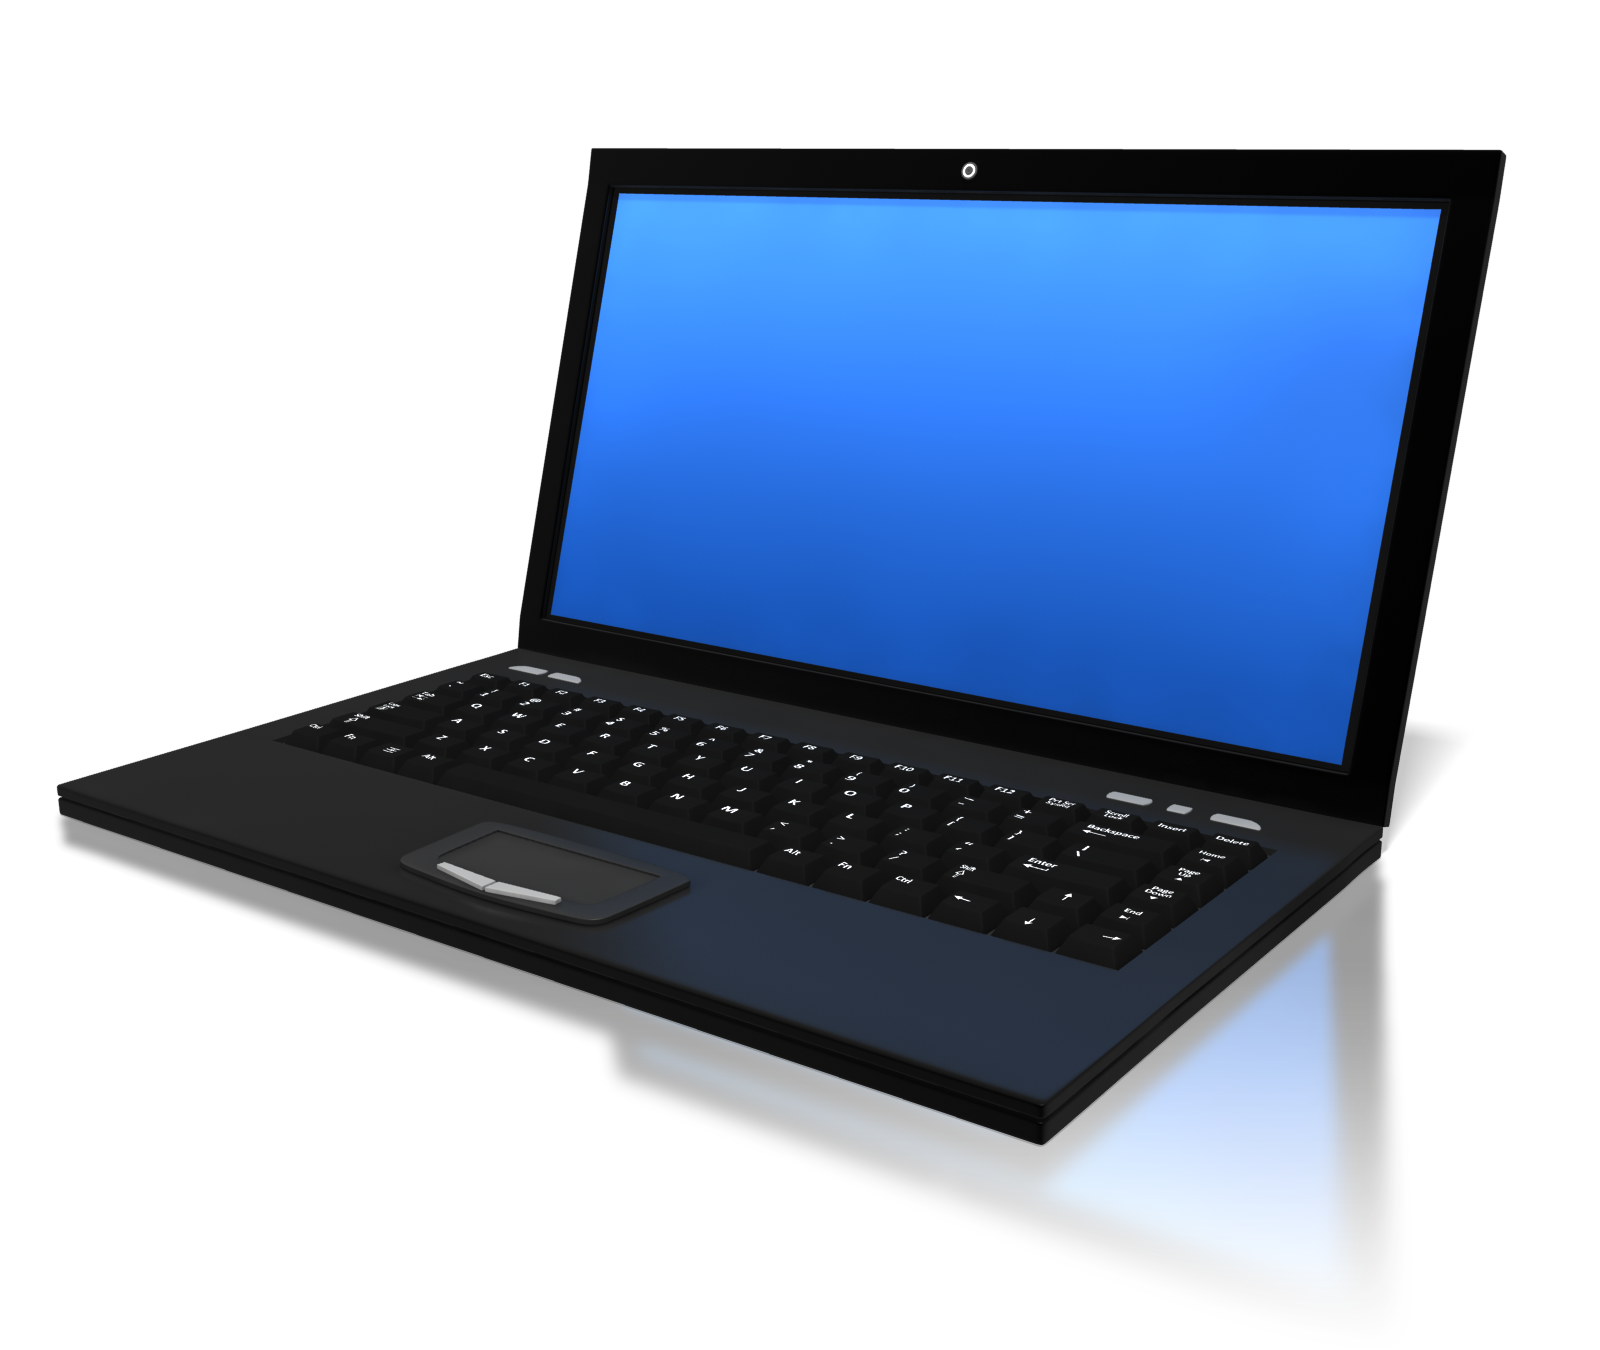
\includegraphics[width=.15\textwidth]{laptop}};
	\node[above right=-0.755 and -0.65 of laptop] () {
\includegraphics[width=.07\textwidth]{key_purple}};

	
	\node[right=5cm of client] (server) {\large AP};
	\node[above = 0 of server] (ap) {
\includegraphics[width=.13\textwidth]{AP}};
	\node[above right=-1.25 and -0.77 of ap] () {
\includegraphics[width=.07\textwidth]{key_purple}};
	
	\coordinate[between = client and server] (midpoint) {};
	\foreach \i in {1, ..., 4} {
		\coordinate[below = \i * \MsgSpace of client] (c\i) {};
		\coordinate[below = \i * \MsgSpace of server] (s\i) {};
	
	}
	
	
	

	\draw[<-, darkgreen] (c1) -- node[above,font=\boldmath] {$N_{AP}$} (s1);
	
	\draw[->, darkgreen] (c2) -- node[above,font=\boldmath] {$N_C,  \mathsf{MAC}(
\includegraphics[width=.06\textwidth, trim=0 7cm 0 0cm]{key_orange}, N_C)$} (s2);

	\draw[<-, darkgreen] (c3) -- node[above,font=\boldmath] {$N_{AP},  \mathsf{MAC}(
\includegraphics[width=.06\textwidth, trim=0 7cm 0 0]{key_orange}, N_{AP})$} (s3);
	
	\draw[->, darkgreen] (c4) -- node[above,font=\boldmath] {$\mathsf{MAC}(
\includegraphics[width=.06\textwidth, trim=0 7cm 0 0]{key_orange}, ``\mathtt{Finished}")$} (s4);	
	
	\node[right = 5pt of s1, yshift=8pt, align=center] {$N_{AP} \gets \bits^{256}$};
	
%	\node[left = 10pt of c1,align=right] (process_C_m2) {
%		$N_C \gets \bits^\secparam$ \\ 
%		$\key_{0} \concat \key_{1} \gets \mathsf{KDF}(
\includegraphics[width=.06\textwidth, trim=0 7.5cm 0 0]{key_purple}, N_C \concat N_{AP})$
%	};

	\node[left = 10pt of c1,align=right] (process_C_m2) {
		$N_C \gets \bits^{256}$ \\
%		$\key_{0} \concat \key_{1} \gets \mathsf{KDF}(
\includegraphics[width=.06\textwidth, trim=0 7.5cm 0 0]{key_purple}, N_C \concat N_{AP})$
		\parbox{0.6cm}{
			
\includegraphics[width=.06\textwidth, trim=0 12cm 0 5cm]{key_orange}\\
			
\includegraphics[width=.06\textwidth, trim=0 7cm 0 -3cm]{key_green}
		} $\gets \mathsf{KDF}(
\includegraphics[width=.06\textwidth, trim=0 7cm 0 0]{key_purple}, N_C \concat N_{AP})$
	};
	
	\node[right = 5pt of s2, align=left] (process_AP_m2) {
		\parbox{0.6cm}{
			
\includegraphics[width=.06\textwidth, trim=0 12cm 0 5cm]{key_orange}\\
			
\includegraphics[width=.06\textwidth, trim=0 7cm 0 -3cm]{key_green}
		} $\gets \mathsf{KDF}(
\includegraphics[width=.06\textwidth, trim=0 7cm 0 0]{key_purple}, N_C \concat N_{AP})$
	};
 	

	
%	\draw[decorate,decoration={brace,amplitude=5pt},thick]  (process_C_m2.north east) --(process_C_m2.south east);

%	\draw[decorate,decoration={brace,amplitude=5pt,mirror,raise=-2pt},thick]  (process_AP_m2.north west) --(process_AP_m2.south west);


	\node[below=0pt of c4] {};
\end{tikzpicture}

}

\end{document}